%\documentstyle[epsf,twocolumn]{jarticle}       %LaTeX2e仕様
%\documentclass[twocolumn]{jarticle}     %pLaTeX2e仕様(platex.exeの場合)
\documentclass[onecolumn]{ujarticle}   %pLaTeX2e仕様(uplatex.exeの場合)
%%%%%%%%%%%%%%%%%%%%%%%%%%%%%%%%%%%%%%%%%%%%%%%%%%%%%%%%%%%%%%
%%
%%  基本バージョン
%%
%%%%%%%%%%%%%%%%%%%%%%%%%%%%%%%%%%%%%%%%%%%%%%%%%%%%%%%%%%%%%%%%
\setlength{\topmargin}{-45pt}
%\setlength{\oddsidemargin}{0cm} 
\setlength{\oddsidemargin}{-7.5mm}
%\setlength{\evensidemargin}{0cm} 
\setlength{\textheight}{24.1cm}
%setlength{\textheight}{25cm} 
\setlength{\textwidth}{17.4cm}
%\setlength{\textwidth}{172mm} 
\setlength{\columnsep}{11mm}

%\kanjiskip=.07zw plus.5pt minus.5pt


% 【節が変わるごとに (1.1)(1.2) … (2.1)(2.2) と数式番号をつけるとき】
%\makeatletter
%\renewcommand{\theequation}{%
%\thesection.\arabic{equation}} %\@addtoreset{equation}{section}
%\makeatother

%\renewcommand{\arraystretch}{0.95} 行間の設定
%%%%%%%%%%%%%%%%%%%%%%%%%%%%%%%%%%%%%%%%%%%%%%%%%%%%%%%%
%\usepackage{graphicx}   %pLaTeX2e仕様(\documentstyle ->\documentclass)
\usepackage[dvipdfmx]{graphicx}
\usepackage{subcaption}
\usepackage{multirow}
\usepackage{amsmath}
%%%%%%%%%%%%%%%%%%%%%%%%%%%%%%%%%%%%%%%%%%%%%%%%%%%%%%%%
\begin{document}
	
	%bibtex用の設定
	%\bibliographystyle{ujarticle} 
	\twocolumn[
	\noindent
	
	\hspace{1em}
	2019 年 7 月 26 日
	ゼミ資料
	\hfill
	M1 寺内 光
	
	\vspace{2mm}
	
	\hrule
	
	\begin{center}
		{\Large \bf 進捗報告}
	\end{center}
	
	
	\hrule
	\vspace{3mm}
	]
	% ‚ここから 文章 Start!
	\section{今週やったこと}
	先週に引き続き Semantic Segmentation 関連の論文を読んでまとめた.
	
	\section{DeepLab \cite{DBLP:journals/corr/ChenPK0Y16, DBLP:journals/corr/abs-1802-02611}}
	Google の出しているオープンソースの Semantic Segmentation のためのモデル.図 \ref{fig:deeplab} にDeepLab v3+ のモデル概要を示す.
	
	\begin{figure}[h]
		\begin{center}
			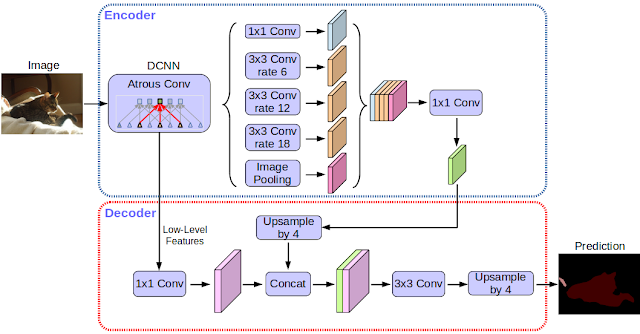
\includegraphics[width=120mm]{deeplab.png}
			\caption{DeepLab モデル概要図}
			\label{fig:deeplab}
		\end{center}
	\end{figure}
	
	現在は DeepLab v3+ が最新バージョン.DeepLab には 3 つの特徴が紹介されている.1 つ目が atrous covolution, 2 つ目が atrous spatial pyramid pooling(ASPP), 3 つ目が CRF による条件付き確率場の利用である.基本的には DCNN と CRF を組み合わせたモデルになっており,DCNN では VGG16 や ResNet を fine tuning したものを用いている.論文では ResNet を用いた時のほうが精度が良かったとある.
	
	\section{atrous convolution}
	拡張畳み込みとも呼ばれる,深い畳み込みニューラルネットワークによって計算された特徴の解像度を明示的に制御し、マルチスケール情報をキャプチャするためにフィルタの視野を調整することを可能にする畳み込み方式.レート r が存在し,r = 1 のときは標準的な畳み込み演算に一致する.特に 2 次元の場合,以下のように定式化される.また,図 \ref{fig:atrous} に概要図を示す.
	
	\begin{equation}
	y[i] = \sum_{k}x[i+r*k]w[k]
	\end{equation}
	
	\begin{figure}[h]
		\begin{center}
			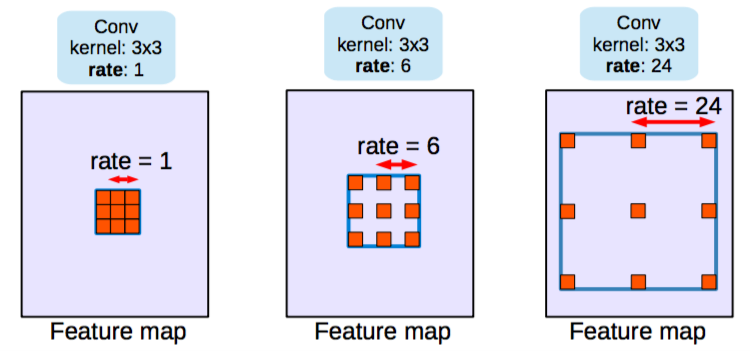
\includegraphics[width=120mm]{atrous.png}
			\caption{atrous 畳み込み概要図}
			\label{fig:atrous}
		\end{center}
	\end{figure}

	\section{atrous spatial pyramid pooling(ASPP)}
	scale invariance を考慮するために atrous 畳み込みのレート r を様々に設定する方法.
	図 \ref{fig:aspp} に ASPP の概要図を示す.様々なレートで畳みこまれたレイヤは重ね合わせて 1×1 の畳み込み演算によって 1 枚のレイヤとなる.
	
	\begin{figure}[h]
		\begin{center}
			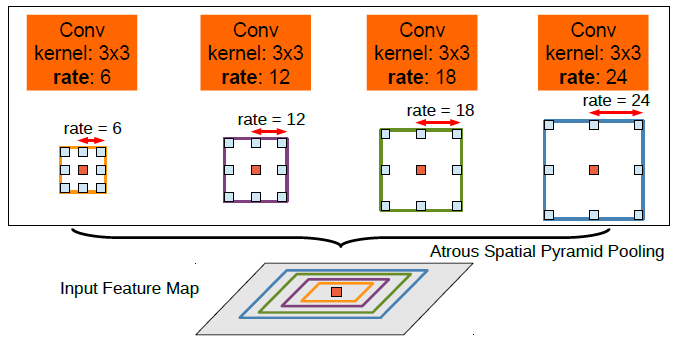
\includegraphics[width=120mm]{aspp.png}
			\caption{ASPP 概要図}
			\label{fig:aspp}
		\end{center}
	\end{figure}

	\section{Conditional Random Field(CRF)}
	CRF は画像の隣り合った画素のペアを考えて,その 2 つが同じ object に入るか否かを計算していく手法である.DeepLab では bilinaer upsampling によって feature map を引きのばし,その直後にfully-connected Conditional Random Field を用いる.下に数式を示す.$\theta_{i}{j}$ における $\mu(x_{i},x_{j})$ はフィルターであり, $x_{i} != x_{j}$ のとき 1 であり,同じときに 0 をとる.カッコ内は重みづけされた 2 つのカーネルの和であり,1つめのカーネルは値の差とピクセルの位置情報を扱い(a kind of bilateral filter),エッジの抽出などを行う.2 つめのカーネルはピクセルの位置情報のみを扱う(Gaussian filter).$\sigma$ と $w$ は cross validation によって得られる.
	\begin{equation*}
	E[x] = \sum_{i}\theta_{i}(x_{i})+\sum_{ij}\theta_{ij}(x_{i},x_{j})\\
	\end{equation*}
	
	\begin{equation*}
	\theta_{i}(x_{i}) = -logP(x_{i})
	\end{equation*}
	
	\begin{eqnarray*}
	\theta_{ij}(x_{i},x_{j}) = \mu(x_{i},x_{j})[w_{1}\exp(-\frac{||p_{i}-p_{j}||^2}{2\sigma_{\alpha}^2}-\frac{||I_{i}-I_{j}||^2}{2\sigma_{\beta}^2})\\+w_{2}\exp(-\frac{||p_{i}-p_{j}||^2}{2\sigma_{\gamma}^2})]
	\end{eqnarray*}
	
	ただし,DeepLab v3, v3+ ではもう使われていない(CRF は前処理が必要で end-to-end な学習ができないため).
	
	\section{来週について}
	github にいろいろなフレームワークでの実装が紹介されているのでひとまず動かせるかどうか試してみたいところではあるが,試験勉強のため来週は進捗お休みします.
	
	% 参考文献リスト
	\bibliographystyle{unsrt}
	\bibliography{2019_07_26_terauchi}
\end{document}